\documentclass[9pt]{pnas-new}
% Use the lineno option to display guide line numbers if required.
% Note that the use of elements such as single-column equations
% may affect the guide line number alignment. 

%\RequirePackage[english,slovene]{babel} % when writing in slovene
\RequirePackage[slovene,english]{babel} % when writing in english

\templatetype{pnasresearcharticle} % Choose template 
% {pnasresearcharticle} = Template for a two-column research article
% {pnasmathematics} = Template for a one-column mathematics article
% {pnasinvited} = Template for a PNAS invited submission

%\selectlanguage{slovene}
%\etal{in sod.} % comment out when writing in english
%\renewcommand{\Authands}{ in } % comment out when writing in english
%\renewcommand{\Authand}{ in } % comment out when writing in english

\newcommand{\set}[1]{\ensuremath{\mathbf{#1}}}
\renewcommand{\vec}[1]{\ensuremath{\mathbf{#1}}}
\newcommand{\uvec}[1]{\ensuremath{\hat{\vec{#1}}}}
\newcommand{\const}[1]{{\ensuremath{\kappa_\mathrm{#1}}}} 

\newcommand{\num}[1]{#1}

\graphicspath{{./fig/}}

\title{Emotion contagion model for dynamical crowd path planning}

% Use letters for affiliations, numbers to show equal authorship (if applicable) and to indicate the corresponding author
\author{Andrej Sušnik}
\author{Timotej Zgonik}
\author{Ema Leila Grošelj}

\affil{Collective behaviour course research seminar report} 

% Introduction, Methods, Results and Discussion

% Please give the surname of the lead author for the running footer
\leadauthor{Sušnik} 

\selectlanguage{english}

% Please add here a significance statement to explain the relevance of your work
% \significancestatement{Procedural generation of a tropic island and \\coral reef}{In computer graphics there is frequent need for displaying large vistas of natural looking terrain. Designing such terrain by hand is typically time consuming. With procedural generation, on the other hand, larger areas of natural looking terrain can be generated with or without minimal intervention in a relatively short time. In this work we present a process of procedural generation of a tropical island with the associated corral reef. We start by generating a heightmap for the base terrain. The heightmap is then transformed by simulating the processes of hydraulic and thermal erosion to achieve a more natural look of the terrain. As coral reefs often grow around tropical islands, we also simulate their growth as part of the last step. Real-time visualization is enabled during the simulation, so that one can observe the evolution of the terrain. Here we dynamically apply textures to the terrain based on its local characteristics. The result is a natural looking model of the textured tropical island and corral reef.}{Procedural generation | Terrain generation | Thermal and hydraulic erosion | Coral reef | Simulation | GPU}

%\selectlanguage{slovene}

% Please include corresponding author, author contribution and author declaration information
%\authorcontributions{Please provide details of author contributions here.}
%\authordeclaration{Please declare any conflict of interest here.}
%\equalauthors{\textsuperscript{1}A.O.(Author One) and A.T. (Author Two) contributed equally to this work (remove if not applicable).}
%\correspondingauthor{\textsuperscript{2}To whom correspondence should be addressed. E-mail: author.two\@email.com}

% Keywords are not mandatory, but authors are strongly encouraged to provide them. If provided, please include two to five keywords, separated by the pipe symbol, e.g:
\keywords{Dynamic crowd path planning | Crowd behavior | Simulation | Emotion contagion} 

\begin{abstract}
An emotion contagion model for dynamical crowd path planning would allow for realistic and plausible simulation of crowd path planning and crowd behavior. Modeling agents' personalities using the OCEAN, or big five, personality trait model allows us to simulate a diverse crowd that reacts to the environment in different ways, while also affecting neighboring agents and their path planning.
\end{abstract}

\dates{\textbf{\today}}
\program{BM-RI}
\vol{2024/25}
\no{CB:GB} % group ID
%\fraca{FRIteza/201516.130}

\begin{document}

% Optional adjustment to line up main text (after abstract) of first page with line numbers, when using both lineno and twocolumn options.
% You should only change this length when you've finalised the article contents.
\verticaladjustment{-2pt}

\maketitle
\thispagestyle{firststyle}
\ifthenelse{\boolean{shortarticle}}{\ifthenelse{\boolean{singlecolumn}}{\abscontentformatted}{\abscontent}}{}

% If your first paragraph (i.e. with the \dropcap) contains a list environment (quote, quotation, theorem, definition, enumerate, itemize...), the line after the list may have some extra indentation. If this is the case, add \parshape=0 to the end of the list environment.

% INTRO
\section{Introduction}
% \dropcap{I}ntroduction: 
Efficient crowd path planning is crucial in various real-world applications, from urban transportation management to emergency evacuations. The \textit{Emotion Contagion Model for Dynamical Crowd Path Planning} article presents an innovative approach by integrating emotional dynamics into crowd behavior modeling, offering a nuanced understanding of how individual emotions influence collective movement patterns.

This article aims to reproduce the results of the original study to validate its findings and explore potential improvements. We would like to see the effect of an agent's emotion memory and how adding an independent panic parameter, distinct from the already existing aggressiveness in that it causes agents to no longer follow the optimal path according to their personality, would affect the simulation.

% METHODS
% \dropcap{M}ethods: 
\section{Methods}
\subsection{Related work}
The \textit{Emotion Contagion Model for Dynamical Crowd Path Planning} article will be the main starting point for our work. The main approach to crowd path planning in the article is shown on the Figure \ref{fig:outline}. 
\begin{figure}[h!]
    \centering
    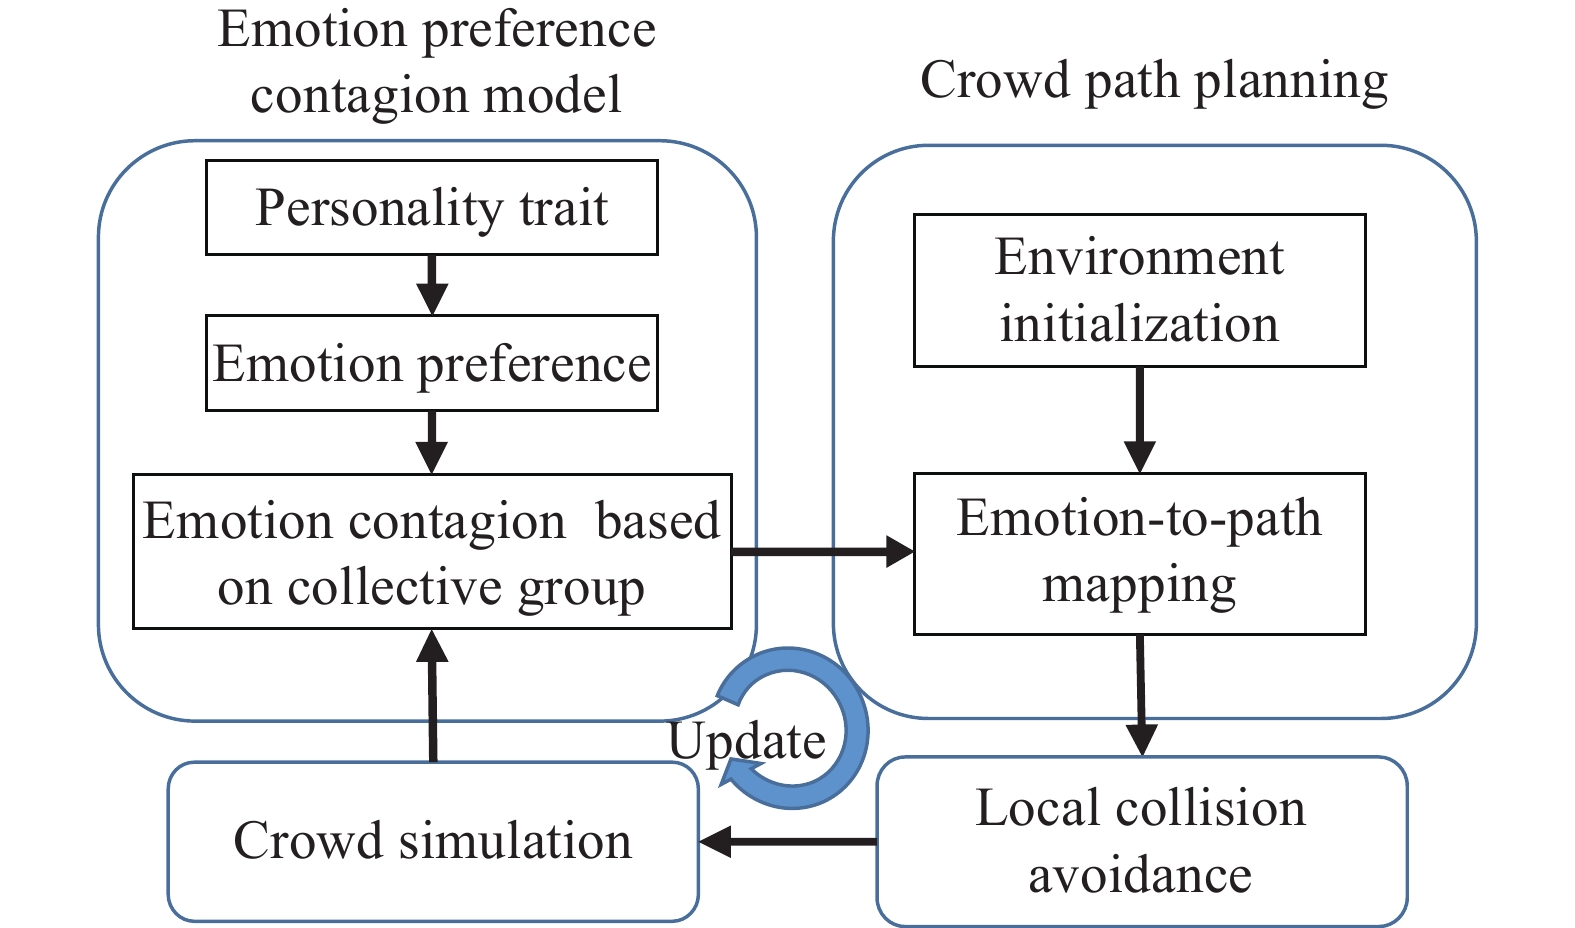
\includegraphics[width=1\linewidth]{fig/outline.jpg}
    \caption{The emotion contagion model as proposed by the source article \cite{Wu_Huang_Tian_Yan_Yu_2024}.}
    \label{fig:outline}
\end{figure}

The source article proposes generating agents with distinct values for the five OCEAN traits: openness to experience, conscientiousness, extroversion, agreeableness, and neuroticism. Based on those factors, agents are then assigned an initial distance preference ${P_d}$ and an initial velocity preference ${P_v}$. Agents have larger distance preferences if their personality factors are simple, aggressive, and fragile (corresponding to OCEAN factors: O${-}$, E${-}$, A${+}$), and agents have larger velocity preferences if their personality factors are variable, energetic, and functional (corresponding to OCEAN factors: C${-}$, E${+}$, N${+}$). If an agent has a large distance preference, its velocity preference is usually smaller, and vice versa. An agent with a larger velocity preference will seek to find less crowded paths even at the cost of the distance being longer, while those with a larger distance preference will stick to a path even as it becomes crowded \cite{Wu_Huang_Tian_Yan_Yu_2024}.

The other aspect of the article is the emotion contagion. For that purpose, the simulation requires a method to define collective clusters among the agents to determine which of them will be mutually affected. Agents are defined as being collective neighbors if they share similar motion and have a mutual goal. Information is contagious between neighboring agents in the same group and is affected by the distance between agents and the difference between emotion preferences. Additionally, agents may be affected by environmental contagious sources, such as a fire disaster \cite{Wu_Huang_Tian_Yan_Yu_2024}.  

The \textit{Simulation of crowd dynamics in pedestrian evacuation concerning panic contagion: A cellular automaton approach} article describes how panic could influence the path planning of the agent.
The authors propose a model where panic is contagious and it negatively impacts the ability of the agent to find an exit.\cite{Wang_2022}
\subsection{Proposed improvements}
% Emotion memory
We propose adding an additional \textbf{Emotion memory} parameter to the agents. The emotion memory parameter would affect the agent on a multi-run simulation where the same agents would be placed in different environments in sequence.


A second improvement that we propose is adding \textbf{Panic contagion} to the simulation. Each agent would have a panic parameter and a panic susceptibility parameter, where panic inhibits the ability of the agent to move to its goal. As the panic parameter increases, the agent movement would become more and more random.

It would also be possible to explore how the clustering algorithm described in the article performs when compared to generalized community detection algorithms, such as Leiden, Walktrap, or (Fast) Label Propagation.


We believe to have found an error in the source article with its equation: \begin{equation*}
    d_{ori}(i,j)=|arccos(vel_i)-arccos(vel_j)|
\end{equation*}
which does not appear to be a operation that can be performed on a vector, so we instead propose: \begin{equation*}
    d_{ori}(i,j)=|atan2(vel_{i_y},vel_{i_x})-atan2(vel_{j_y},vel_{j_x})|
\end{equation*}
where we obtain the correct angle ${\theta}$\ from the \textit{x}-axis \cite{wikiatan2} for each of a pair of agents and then subtract the angles to obtain the difference between their orientations.
\cite{Wu_Huang_Tian_Yan_Yu_2024}
% RESULTS
\section{Results}
We have implemented a basic simulation showing the effects of the clustering algorithm. Figure \ref{fig:enter-label} shows multiple runs of the clustering algorithm.

\begin{figure}[h!]
    \centering
    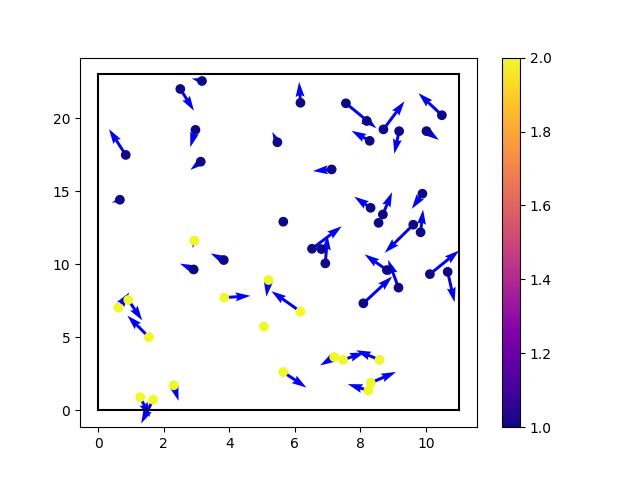
\includegraphics[width=0.3\linewidth]{fig/Figure_2.png}
    \hfill
    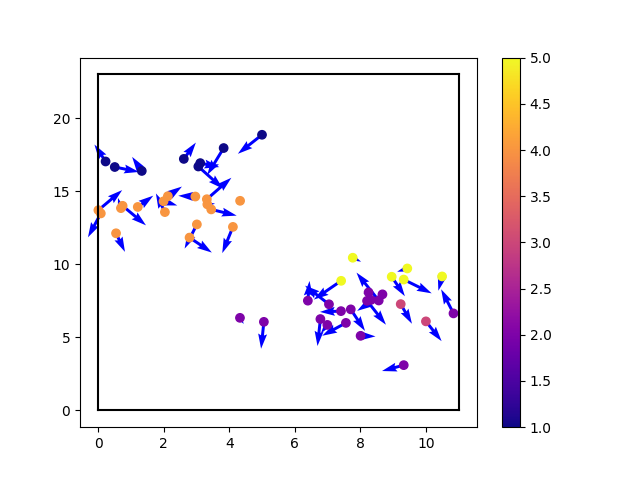
\includegraphics[width=0.3\linewidth]{fig/Figure_3.png}
    \hfill
    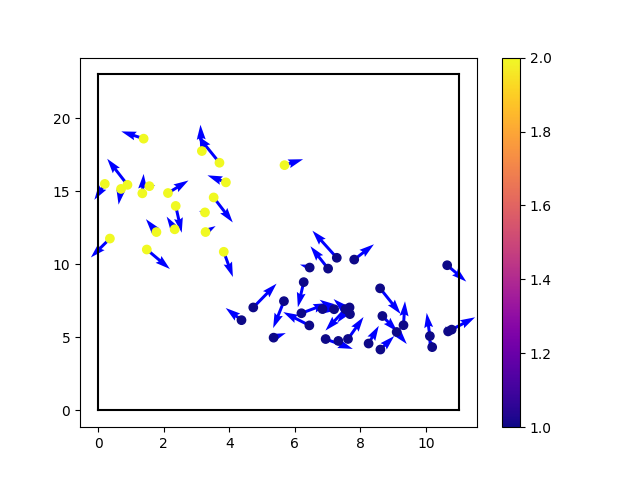
\includegraphics[width=0.3\linewidth]{fig/Figure_4.png}
    \caption{Example runs of clustering according to association with the closest neighbor with a higher degree. The implementation is currently slightly unstable, but it may suffice for the purpose of emotion contagion. The leftmost sub-figure represents agents with positions initialized uniformly, while the two to the right represent agents with positions initialized with a bimodal Gaussian distribution.}
    \label{fig:enter-label}
\end{figure}

% DISCUSSION
\section{Discussion}
At this stage, we have implemented a simple simulation workflow where we can define the environment in the text format and then run the simulation with specified number of agents. By the next submission deadline, we plan to have implemented the simulation from the original article in its entirety, as well as specifying how to integrate the proposed additions to its model.
% \dropcap{D}iscussion: .... ljanja morebitnih ostalih objektov, kot so drevesa in skale. Ker je v primeru večjih terenov proceduralno generiranje mnogokrat računsko intenzivna operacija, posamezne korake implementiramo na grafični procesni enoti (GPE), ki je zaradi njene visoko paralelne arhitekture zmožna hitrega procesiranja velike količine podatkov. Najprej generiramo začetni teren, nato pa za bolj verodostoje

% \clearpage

% \dropcap{D}iplomsko delo prikazuje metode za proceduralno generiranje tropskega otoka, primernega za uporabo v računalniški igri. Omejimo se na generiranje in teksturiranje terena, brez postavljanja morebitnih ostalih objektov, kot so drevesa in skale. Ker je v primeru večjih terenov proceduralno generiranje mnogokrat računsko intenzivna operacija, posamezne korake implementiramo na grafični procesni enoti (GPE), ki je zaradi njene visoko paralelne arhitekture zmožna hitrega procesiranja velike količine podatkov. Najprej generiramo začetni teren, nato pa za bolj verodostojen videz simuliramo hidravlično in termično erozijo. Ker v tropskih morjih v okolici otokov običajno rastejo koralni grebeni, izvedemo tudi simulacijo rasti le-teh. Na teren lepimo teksture ustrezne njegovim značilnostim. 

% Enega pomembnejših prispevkov na področju proceduralnega generiranja je naredil Ken Perlin. Predstavil je način generiranja šuma, ki ga danes imenujemo Perlinov šum \cite{perlin_noise_85}. Perlinov šum se uporablja na mnogo področjih, eno izmed njih pa je proceduralna gradnja terena. Perlin je kasneje predstavil še šum \emph{Simplex} \cite{simplex_noise_01}, ki je za izračun hitrejši in še dodatno izboljša videz. V delu za gradnjo začetnega terena uporabljamo slednjega, ker še danes predstavlja najboljši kompromis med hitrostjo izračuna, pomnilno potratnostjo in kvaliteto \cite{rose2016algorithms}.

% Musgrave, Kolb in Mace \cite{synthesis_first_89} so eni izmed prvih, ki so predstavili simuliranje erozije. Opisujejo tako termično kot tudi hidravlično erozijo in način prikaza generiranega terena. Hidravlična erozija simulira pretakanje vode po terenu, ki spodjeda material, ga prenaša v svojem toku in nato odlaga. Termična erozija pa zajema dejavnike, ki drobijo površino terena v drobir, ta pa nato drsi po strmih pobočjih. Simuliranje hidravlične erozije sta predstavila tudi Beneš in Forsbach \cite{benevs_first_02}. Mei, Decaudin in Hu \cite{benevs_fast_gpu_07} pa so prvi predstavili implementacijo hidravlične erozije iz \cite{benevs_first_02} na GPE. Jákó in Tóth \cite{jako_fast_gpu_11} sta dodatno opisala še implementacijo termične erozije na GPE. Generiranje terena s pomočjo hidravlične in termične erozije na GPE je v svojem diplomskem delu opisal tudi Maške \cite{maske_2013}. V tem delu uporabljamo drugačen pristop k generiranju začetnega terena kot ostali in po simulaciji erozije simuliramo še rast koralnega grebena ter na teren nanesemo teksture.

% Virov, ki prikazujejo simuliranje rasti koral z namenom vizualizacije v računalniški grafiki nismo našli. Po drugi strani pa smo našli vira, ki predstavljata model rasti koral in s tem koralnega grebena namenjen znanstvenim raziskavam \cite{nakamura_reef_model_07,nakamura_reef_simulation_11}. Z nekaj poenostavitvami smo ta model priredili našim potrebam.

% \section*{Metode}
% Za predstavitev terena smo uporabili višinsko karto (angl. \emph{heightmap}). To je rastrska slika, kjer vsak piksel predstavlja višino v pripadajoči točki na terenu. 

% \subsection*{Generiranje začetnega terena}
% Ker je bil cilj generirati teren v obliki otoka smo želeli, da bo teren na sredini višinske karte višji kot ob robovih. To smo dosegli z generiranjem višinske karte, ki definira teren v obliki stožca z nelinearno klančino:
% \begin{equation} \label{eq:stozec}
% h_\mathrm{A}(x,y) =   
% \begin{cases}
% \const{H} \left(1-\left(\frac{r(x,y)}{\const{R}}\right)^\const{P}\right); &\text{če } r(x,y) < \const{R}\\
% 0; &\text{sicer,} \\
% \end{cases}
% \end{equation}
% kjer $\const{H}$ označuje višino stožca, $\const{R}$ polmer stožca in $\const{P}$ potenco, ki nadzoruje obliko klančine,
% \begin{equation} \label{eq:dist_to_center}
% r(x,y) = \sqrt{(x - x_\mathrm{C})^2 + (y - y_\mathrm{C})^2}
% \end{equation}
% pa razdaljo točke $(x,y)$ do središča osnovne ploskve stožca $(x_\mathrm{C},y_\mathrm{C})$.

% Za izboljšanje verodostojnosti terena smo v naslednjem koraku generirali dodatno višinsko karto, ki smo jo potem združili s prvo. Za generiranje te smo uporabili šum Simplex \cite{simplex_noise_01}, ki ga lahko implementiramo v poljubno mnogo dimenzijah in s katerim lahko dosežemo hribovit videz. V naši rešitvi uporabljamo C\# implementacijo, ki je del prosto dostopnega paketa MinePackage\footnote{\href{https://sourceforge.net/projects/minepackage/}{sourceforge.net/projects/minepackage}}. Za boljši videz terena smo uporabili več oktav šuma\footnote{\href{http://www.redblobgames.com/maps/terrain-from-noise/}{www.redblobgames.com/maps/terrain-from-noise}}. Izraz oktava v glasbeni teoriji označuje interval med višinama dveh tonov, od katerih ima eden dvojno oziroma polovično frekvenco drugega. V primeru funkcije šuma z višanjem frekvence šuma (skala šuma) zmanjšujemo tudi amplitudo. Na eni višinski karti smo uporabili več oktav šuma tako, da smo vse oktave skupaj sešteli: 
% \begin{equation} \label{eq:octaves_simplex}
% h_\mathrm{B}(x,y) = \sum_{i=0}^{N} \eta(x 2^i, y 2^i) \frac{1}{2^i},
% \end{equation}
% kjer je $\eta$ vrednost šuma Simplex v koordinatah $(x,y)$ in $N$ število oktav.

% Pri združevanju višinskih kart stožca in šuma smo se zgledovali po orodju Worldmachine\footnote{\href{http://www.world-machine.com/}{www.world-machine.com}}, kjer je možno več višinskih kart združiti v eno na več načinov. Najboljše rezultate smo dobili, ko smo višinski karti združili s potenciranjem:
% \begin{equation} \label{eq:map_merge}
% h_\mathrm{C}(x,y) = h_\mathrm{A}(x,y)^{1 + h_\mathrm{B}(x,y)\const{N}},
% \end{equation}
% kjer je $h_\mathrm{A}$ višina v višinski karti stožca, $h_\mathrm{B}$ pa višina v višinski karti šuma Simplex. Vpliv šuma določa parameter $\const{N}$.

% Ker smo želeli, da otok dobi videz vulkana, smo dodali možnost generiranja vulkanskega kraterja. Generirali smo ga tako, da smo vse vrednosti v združeni višinski karti $h_\mathrm{C}$, ki so višje od določenega praga, preko praga preslikali navzdol. Postopek prikazuje enačba (\ref{eq:crater}), kjer je $h$ končna višinska karta začetnega terena, $\const{C}$ pa višina pragu in s tem višina, na kateri se ustvari vulkanski krater. Slika \ref{fig:merged_crater_example} pa prikazuje relief generiran z uporabo končne višinske karte začetnega terena.

% \begin{equation} \label{eq:crater}
% h_0(x,y) = 
% \begin{cases}
% 2\const{C} - h_\mathrm{C}(x,y); & \text{če } h_\mathrm{C}(x,y) > \const{C}\\
% h_\mathrm{C}(x,y); & \text{sicer}\\
% \end{cases}
% \end{equation}

% \begin{figure}
% 	\centering
% 	\includegraphics[width=.8\linewidth]{example_merged_crater_screen}
% 	\caption{Začetni relief terena.}
% 	\label{fig:merged_crater_example}
% \end{figure}

% \subsection*{Erozija}
% Kljub temu, da že začetni teren spominja na otok, je njegov videz še neprepričljiv. Simuliranje naravnih procesov, kot sta hidravlična in termična erozija, nam omogoča videz izboljšati. Hidravlično erozijo smo implementirali po viru \cite{benevs_fast_gpu_07}, termično pa po \cite{jako_fast_gpu_11}. Vira opisujeta metodi simuliranja teh procesov na GPE.

% \subsubsection*{Hidravlična erozija}
% Simuliranje hidravlične erozije se začne s simuliranjem pretakanja vode po površini terena. Na podlagi hitrosti vode in naklona terena določimo količino raztopljenega sedimenta ter njegov prenos. V predelih hitrejšega vodnega toka voda teren odnaša, v počasnejših pa odlaga. S tem se teren preoblikuje in dobi želen erodiran videz. Voda med simulacijo ves čas izhlapeva.

% Za opis simulacije bomo uporabljali naslednje pomembne količine: višina terena, količina tekoče vode, količina razstopljenega sedimenta, odtočni tokovi vode, in hitrost vode. Pri tem se vsaka od količin hrani za vsako točko (celico) terena. S $t$ dodatno označujemo trenutni čas in s $\tau$ časovni korak ene iteracije simulacije. Vsaka iteracija je razbita na več zaporednih korakov: dodajanje vode, pretakanje vode po terenu, izračun odloženega in stopljenega sedimenta, prenos sedimenta, difuzija sedimenta, izhlapevanje vode. Vsak korak uporabi količine iz prejšnjega in jih posodobi. Nekatere količine se izračunajo v večih podkorakih, zato te indeksiramo z $'$, $''$ itd., da med seboj ločimo vrednosti v različnih podkorakih. Sosednje celice trenutne celice ozačujemo z L (leva), R (desna), T (gornja), B (spodnja).

% Za simuliranje pretakanja vode uporabljamo prirejen model, ki povezuje sosednje celice z navideznimi cevmi, po katerih se med njimi izmenjuje voda \cite{splashing_fluids_95}. Ob začetku simulacije privzemamo, da je višina vode po celotnem terenu ničelna; $d_0=0$. Dež predstavlja nastanek nove vode, kar za obravnavano celico $(x,y)$ izračunamo kot
% \begin{equation} \label{eq:new_water}
% {d_{t}}' = d_t + r \tau,
% \end{equation}
% kjer $r$ označuje količino dežja, ki prispe v celico na enoto časa. Zaradi velikosti terena namreč ni smiselno simulirati dežja kot posameznih kapelj, temveč kot uniformno rast količine tekoče vode po posamezni celici terena. 

% Za vsako celico hranimo njene odtočne tokove $L, R, T, B$ do štirih sosednjih celic, njeni pritočni tokovi pa so ustrezni odtočni tokovi obravnavani celici sosednjih celic. V vsaki iteraciji simulacije se tok vode v odtočnih tokovih pospeši zaradi razlike v hidrostatičnem tlaku med celicami, količina tekoče vode pa se nato izračuna s kopičenjem vseh tokov v virtualnih ceveh. 

% Odtočni tok v smeri proti levi celici za obravnavano celico izračunamo po enačbi: 
% \begin{equation} \label{L0}
% {L_{t}}' = \max\left\{0, L_t + \tau\const{A} \frac{\const{g} \Delta h^\mathrm{L}_t}{\ell} \right\},
% \end{equation}
% kjer $\const{A}$ predstavlja površino prereza cevi, $\ell$ dolžino cevi med dvema sosednjima celicama, $\const{g}$ gravitacijski pospešek in $\Delta h^\mathrm{L}_t$ razliko višin med obravnavano ter levo sosednjo celico $(x-1, y)$, ki se izračuna po enačbi:
% \begin{equation}
% \Delta h^\mathrm{L}_t = h_t + {d_{t}}' - h^\mathrm{L}_t - {d^\mathrm{L}_{t}}'.
% \end{equation}

% Odtočni tokovi v smeri sosed R, T, B se izračunajo na enak način. Ker izračun odtočnih tokov upošteva višinske razlike do vsake sosede individualno, obstaja možnost, da bi iz obravnavane celice odteklo več vode, kot je ta vsebuje. S tem bi količina tekoče vode v celici po izračunu postala negativna. Težavo se rešuje z omejitvijo moči vsakega izmed odtočnih tokov v odvisnosti od količine tekoče vode v celici in predvidene moči vseh odtočnih tokov \cite{benevs_fast_gpu_07,maske_2013}. V primeru odtočnega toka v smeri proti levi celici se tako odtočni tok v naslednjem koraku simulacije izračuna kot:
% \begin{equation}
% L_{t+\tau} = {L_t}' \min\left\{1, \frac{{d_{t}}' \ell^2}{\tau \sum {\set{O}_t}'}\right\},
% \end{equation}
% kjer ${\set{O}_t}'$ predstavlja množico vseh odtočnih tokov obravnavane celice $\left\{{L_t}', {R_t}', {T_t}', {B_t}'\right\}$ izračunanih z uporabo enačbe \eqref{L0}, $\sum {\set{O}_t}'$ pa njihovo skupno vsoto.

% Pretakanje vode po navideznih ceveh se odraža v spremembi količine tekoče vode
% \begin{equation}
% {d_{t}}'' = {d_{t}}' + \frac{\sum \set{I}_{t + \tau} - \sum \vec{O}_{t + \tau}}{\ell^2} \tau,
% \end{equation}
% kjer sta $$\set{I}_{t + \tau} = \left\{R^\mathrm{L}_{t + \tau}, L^\mathrm{R}_{t + \tau}, B^\mathrm{T}_{t + \tau}, T^\mathrm{B}_{t + \tau}\right\}$$ in $$\set{O}_{t + \tau} = \left\{L_{t + \tau}, R_{t + \tau}, T_{t + \tau}, B_{t + \tau}\right\}$$ po vrsti množici pritočnih in odtočnih tokov obravnavane celice v naslednjem časovnem koraku. Pri simuliranju pretakanja vode moramo upoštevati robne pogoje, ki izhajajo iz dejstva da je teren končen. Iztekanje vode s terena omejimo tako, da vsaki cevi, ki nima sosednje celice, postavimo vrednosti ustreznih odtočnih in pritočnih tokov na 0. Na primer: za celice brez levega soseda $(0,y)$ postavimo tako levi odtočni tok $L$, kot tudi desni pritočni tok $R^\mathrm{L}$ na 0.

% Voda med pretakanjem zaradi erozije pretvori del terena v sediment
% \begin{equation} \label{eq:sediment_capacity}
% S = \kappa_\mathrm{S} \left\| \vec{v}_t \right\| \sin{\alpha},
% \end{equation}
% ki ga nato prenaša in odlaga po terenu. V enačbi \eqref{eq:sediment_capacity} $\kappa_\mathrm{S}$ predstavlja konstanto kapacitete sedimenta, $\alpha$ pa lokalni naklon terena v celici. Slednjega za obravnavano celico izračunamo kot $\alpha  = \arccos(\uvec{n}_t \cdot \vec{k})$. Pri tem $\uvec{n}_t$ predstavlja normalo na teren, ki jo pridobimo kot
% \begin{equation}
% \vec{m} = \vec{i}\frac{h^{\mathrm{R}}_t - h^{\mathrm{L}}_t}{\const{M}} + \vec{j}\frac{h^{\mathrm{T}}_t - h^{\mathrm{B}}_t}{\const{M}} + \vec{k},
% \quad
% \uvec{n}_t = \frac{\vec{m}}{\left\|\vec{m}\right\|},
% \end{equation}
% kjer je $\const{M}$ razalja med sosednjimi celicami terena, $\vec{i}$, $\vec{j}$, $\vec{k}$ pa po vrsti enotski vektorji, ki kažejo v smereh osi x, y in z. Hitrost vode v obravnavani celici $\vec{v}_t = \langle v_\mathrm{x}, v_\mathrm{y} \rangle$, ki jo potrebujemo v enačbi \eqref{eq:sediment_capacity} pa izračunamo s pomočjo odtočnih in pritočnih tokov celice:
% \begin{eqnarray} \label{eq:velocity1}
% v_\mathrm{x}=\frac{R^\mathrm{L}_{t+\tau} - L_{t+\tau} + R_{t+\tau} - L^\mathrm{R}_{t+\tau}}{\ell ({d_t}' + {d_t}'')}, \\
% v_\mathrm{y}=\frac{T^{\mathrm{B}}_{t+\tau} - B_{t+\tau} + T_{t+\tau} - B^{\mathrm{T}}_{t+\tau}}{\ell ({d_t}' + {d_t}'')}.
% \end{eqnarray}

% Na zelo položnih delih, kjer se $\alpha$ približuje 0, je vrednost $S$ zelo nizka. Na takšnih predelih proces erozije ne bo imel občutnega učinka. To lahko omilimo na tak način, da $\alpha$ navzdol omejimo s poljubno minimalno vrednostjo. Na podlagi vrednosti $S$ in raztopljenega sedimenta iz predhodne iteracije simulacije, $s_t$, se odločimo, ali se bo del sedimenta odložil ter pretvoril nazaj v teren ali ne. Ko velja $S > s_t$, se zgodi proces erozije in del terena se raztopi, v nasprotnem primeru se del raztopljenega sedimenta odloži in pretvori nazaj v teren. Novo višino terena in količino raztopljenega sedimenta izračunamo po enačbah:
% \begin{eqnarray}
% h_{t+\tau} = 
% \begin{cases}
% h_t - \kappa_\mathrm{E} (S - s_t); &\text{če } S > s_t\\
% h_t + \kappa_\mathrm{D} (S - s_t); &\text{sicer}
% \end{cases}\\
% {s_{t}}' =
% \begin{cases}
% s_t + \kappa_\mathrm{E} (S - s_t); &\text{če } S > s_t\\
% s_t - \kappa_\mathrm{D} (S - s_t); &\text{sicer,}\\
% \end{cases}
% \end{eqnarray}
% kjer je $\kappa_\mathrm{E}$ konstanta topljenja materiala, $\kappa_\mathrm{D}$ pa konstanta odlaganja materiala.

% Raztopljeni sediment prenaša vodni tok, kar opisuje advekcijska enačba $\frac{\delta s}{\delta t} + (\vec{v}_t \nabla s) = 0$.
% Enačbo rešujemo z Eulerjevim korakom nazaj v času, kar pomeni da količini raztopljenega sedimenta v obravnavani celici $(x,y)$ priredimo vrednost, ki je odvisna od vodnega toka v njej
% \begin{equation}
% {s_{t}}''(x,y) = {s_{t}}'(x - v_\mathrm{x} \tau, y - v_\mathrm{y} \tau),
% \end{equation}
% kjer koordinate $(x - v_\mathrm{x} \tau, y - v_\mathrm{y} \tau)$ omejimo na območje terena. Kot je že Maške \cite{maske_2013} omenil, postopek ne deluje zadovoljivo saj je možno, da se v enem koraku količina sedimenta iz ene celice preslika v več celic. Opazili smo tudi, da se sediment pri nižjih hitrostih vode večkrat prenaša v ravnih črtah. Vzrok za to je, da se sediment v območjih nizke hitrosti prenaša med celicami, ki so neposredne sosede. To daje polju sedimenta grob in nenaraven videz, zato ga mi dodatno gladimo s simuliranjem difuzije sedimenta. 

% Difuzijo simuliramo z dvodimenzionalno Laplacevo enačbo, ki jo numerično rešujemo z Jakobi iteracijami \cite{laplace_gpu}. Izračun iteracije prikazuje enačba 
% \begin{equation} \label{eq:jakobi_iter}
% s_{t+\tau} = \frac{{s^\mathrm{L}_{t}}'' + {s^\mathrm{R}_{t}}'' + {s^\mathrm{T}_{t}}'' + {s^\mathrm{B}_{t}}''}{n_\mathrm{W}},
% \end{equation}
% kjer $n_\mathrm{W}$ predstavlja število celic izmed L, R, T in B, ki držijo vodo (${d_{t}}'' > 0$). Robne pogoje smo poenostavili tako, da se koordinate celic omejijo na območje terena. Na primer: za vse celice, ki ležijo na levem robu terena $(0, y)$, se koordinate leve sosednje celice $(x-1, y)$ omejijo na $(0, y)$. Celicam, ki ne vsebujejo vode, nastavimo vrednost ${s_{t}}''$ na 0.

% V zadnjem koraku vsake iteracije simulacije hidravlične erozije upoštevamo, da se količina tekoče vode spreminja tudi zaradi izhlapevanja. V našem delu predpostavljamo, da je temperatura ozračja med simulacijo konstantna, zato hitrost izhlapevanja določamo s konstanto $\kappa_\mathrm{T}$. Proces izhlapevanja opisuje enačba
% \begin{equation}
% d_{t + \tau} = {d_{t}}''(1 - \const{T} \tau).
% \end{equation}

% \subsubsection*{Termična erozija}
% Hidravlična erozija oblikuje grob teren z veliko ostrimi robovi, kar je opazno predvsem na pobočjih ob vodnih strugah, ki se neprestano poglabljajo. S simuliranjem termične erozije, ki modelira proces razgradnje kamnin v drobir zaradi temperaturnih sprememb in njegovo nadaljne razsipanje, teren zgladimo in izboljšamo njegov videz. Podobno kot za hidravlično lahko tudi za termično erozijo uporabljamo model virtualnih cevi, le da v tem primeru cevi prenašajo drobir (terena) namesto vode. Vendar se običajno \cite{jako_fast_gpu_11,maske_2013} zaradi boljšega rezultata pri termični eroziji namesto von Neumannove okolice, ki zaobjema zgolj najbližje štiri sosede obravnane celice, uporablja Moorova okolica, ki zajema vseh osem najbližjih sosednjih celic $\set{N} \in \left\{\mathrm{L},\mathrm{R},\mathrm{T},\mathrm{B}, \mathrm{TL},\mathrm{TR},\mathrm{BL},\mathrm{BR}\right\}$. To bi lahko sicer storili že pri hidravlični eroziji, vendar menimo, da bi povzdignilo kompleksnost implementacije brez večjih izboljšav pri rezultatu. 

% Količina drobirja, ki jo lahko v eni iteraciji prenesemo v vsako od sosednjih celic, je omejena z $M_t = \frac{H_t}{2} \tau \const{M}^2$, kjer je $H_t = h_t - \min\left\{ h^i_t|\ i \in \set{N} \right\}$ razlika v višini terena v obravnavani celici in najnižjo višino terena v njej sosednjih celicah. Če to vrednost presežemo, začne algoritem oscilirati \cite{jako_fast_gpu_11}. Nadaljni proces smo glede na vir \cite{jako_fast_gpu_11} nekoliko poenostavili; vir upošteva tudi lokalno trdnost terena, ki je v našem delu ne.

% Drobir se pod vplivom gravitacije razsipa med nižje ležeče sosednje celice, ki z obravnavano celico tvorijo kot naklona, večji od kota mirovanja $\const{\alpha}$. To je kritičen kot pobočja, ki ga lahko nek zrnat material še tvori. Kadar klančina preseže kot mirovanja, material zdrsne. %V praksi ga izmerimo tako, da material počasi sipamo med dve prozorni plošči in opazujemo kot klančine, ki pri tem nastane.

% Kote naklona med obravnavano in posamezno sosednjo celico $i \in \set{N}$ izračunamo kot $\alpha^i_t = \arctan \frac{h_t - h_t^i}{\const{M}}$.
% Na podlagi teh sestavimo množico, ki vsebuje vse sosednje celice z naklonom, večjim od kota mirovanja $\const{\alpha}$:
% \begin{equation}
% \set{R}_t =\left\{i \in \mathbf{N}|\ \alpha^i_t > \const{\alpha}\right\}.
% \end{equation}

% V vsako celico iz množice $\set{R}_t$ na podlagi višinske razlike z obravnavano celico prenesemo temu proporcionalno količino drobirja, v ostale celice ga ne prenašamo. Na primer: količino drobirja, ki se prenese v levo sosednjo celico, če ta spada v množico $\set{R}_t$, izračunamo z enačbo:
% \begin{equation}
% L_t = M_t \frac{h^\mathrm{L}_t}{\sum_{i \in \set{R}_t}h^i_t}.
% \end{equation}

% \begin{figure}
% 	\centering
% 	\includegraphics[width=.8\linewidth]{example_erosion_screen}
% 	\caption{Relief terena po hidravlični in termični eroziji.}
% 	\label{fig:finished_erosion}
% \end{figure}

% Zaradi paralelnega izvajanja simulacije drobirja ne prestavimo v celice takoj, temveč za ta proces uporabimo navidezne cevi. Končno višino vsake celice izračunamo podobno kot pri hidravlični eroziji, in sicer tako, da k trenutni višini prištejemo vse pritočne tokove in odštejemo vse odtočne:
% \begin{equation}
% h_{t+\tau} = h_t + \sum \set{M}^\mathrm{in}_t - \sum \set{M}^\mathrm{out}_t,
% \end{equation}
% le da tokrat z
% $$\set{M}^\mathrm{out}_t=\left\{ L_t,R_t,T_t,B_t,\mathit{TL}_t,\mathit{TR}_t,\mathit{BL}_t,\mathit{BR}_t \right\}$$
% označimo drobir, ki se iz obravnavane celice razsipa v sosednje celice preko ustreznih virtualnih cevi (odtočni tokovi drobirja), z $$\set{M}^\mathrm{in}_t=\langle R^\mathrm{L}_t, L^\mathrm{R}_t,\ldots,\mathit{TL}^\mathrm{BR}_t \rangle$$
% pa pritočne tokove drobirja (odtočne tokove drobirja usreznih sosed). Primer terena po končani simulaciji prikazuje slika \ref{fig:finished_erosion}.

% \subsection*{Rast koralnega grebena}
% V tropskih morjih okoli otokov, predvsem takšnih vulkanskega nastanka, velikokrat rastejo korale, ki skozi čas tvorijo koralne grebene \cite{oxford_encly_1995}. Korale rastejo v plitvinah toplejših morij. Za rast potrebujejo svetlobo, saj ožigalkarji živijo v sožitju s fotosinteznimi algami zooksantele (angl. \emph{zooxanthellae}) \cite{oxford_encly_1995}. Sestavljene so iz kolonij majhnih polipov, katerih apnenčasti zunanji skeleti se nalagajo in tvorijo koralne grebene. K tvorbi grebena pripomorejo tudi ostali organizmi, ki živijo v koralnem ekosistemu. S simuliranjem rasti koralnih grebenov želimo videz otoka še bolj približati resničnosti in ga narediti zanimivejšega.

% Model rasti koralnega grebena predstavljen v nadaljevanju temelji na modelu Nakamure in Nakamorija \cite{nakamura_reef_simulation_11}. Avtorja sta predstavila model rasti koralnega grebena na podlagi intenzitete svetlobe ter koncentracije anorganskega ogljika v vodi, a za dvodimenzionalne simulacije rasti v pogledu s strani. Ker za naše potrebe potrebujemo pristop, s katerim je mogoče rast simulirati v pogledu iz zraka, smo njun model priredili in poenostavili.

% V opisu bomo uporabljali dve pomembni količini: višina terena (morskega dna) in koncentracija anorganskega ogljika v vodi. Obe količini se hranita za vsako točko oziroma celico terena. Vsaka iteracija simulacije pa je razbita na dva zaporedna koraka; rast koral in difuzijo koncentracije anorganskega ogljika. 

% Kalcifikacija koral je v veliki meri odvisna od stopnje fotosinteze, ki jo lahko izračunamo na podlagi globine vode
% \begin{equation} \label{eq:depth}
% g_t = w_t - h_t,
% \end{equation}
% kjer $w_t$ označuje globalno višino morske gladine v trenutni iteraciji simulacije. Korale zaradi plimovanja in ostalih dejavnikov namreč običajno rastejo le do določene globine vode $\const{G}$. Stopnjo kalcifikacije koral izračunamo z uporabo enačbe
% \begin{equation} \label{eq:calcification_rate}
% c_t=
% \begin{cases}
% O_t^2 \kappa_\mathrm{B} e^{-g_t\const{A}}; & \text{če } g_t < \const{G} \\
% 0; & \text{sicer,} \\
% \end{cases}
% \end{equation}
% kjer je $O_t$ vrednost koncentracije anorganskega ogljika v vodi v trenutni iteraciji simulacije, $\const{B}$ konstanta hitrosti kalcifikacije in $\const{A}$ konstanta absorbcije vode. V prvi iteraciji simulacije je vrednost $O_t$ vsake celice postavljena na $O_0$.

% Korale za rast porabijo določeno količino anorganskega ogljika, zato moramo vrednost njegove koncentracije v vodi zmanjšati v sorazmerju s stopnjo kalcifikacije. Spremembo izračunamo po enačbi
% \begin{equation} \label{eq:ct_deplete}
% {O_t}' = \max\left\{0, O_t - \frac{c_t\tau}{g_t} \const{U} \right\}, 
% \end{equation}
% kjer $\const{U}$ nadzoruje stopnjo porabe anorganskega ogljika. S tem, da v enačbi \eqref{eq:ct_deplete} stopnjo kalcifikacije delimo z višino vode,  dosežemo, da se pri enaki stopnji rasti koral koncentracija anorganskega ogljika v vodi zmanjša primerno količini vode nad to točko na terenu.

% Na koncentracijo anorganskega ogljika v vodi vpliva tudi plimovanje in mešanje vode. Ker v našem primeru simulacija teče v časovnem razponu več tisoč let in to na velikem terenu, lahko ta vpliv prikažemo s preprosto difuzijo, podobno kot smo to storili s sedimentom pri hidravlični eroziji
% \begin{equation} \label{eq:ct_diffusion_jacobi}
% O_{t + \tau} = \frac{{O^\mathrm{L}_{t}}' + {O^\mathrm{R}_{t}}' + {O^\mathrm{T}_{t}}' + {O^\mathrm{B}_{t}}'}{n_\mathrm{U}},
% \end{equation}
% kjer $n_\mathrm{U}$ predstavlja število najbližjih sosednjih celic v von Neumannovi okolici, ki ležijo pod morsko gladino ($g_t > 0$) \cite{laplace_gpu}. Pri robnih celicah, celicah, ki ležijo tik ob robu terena in zato nimajo levega ali desnega, ali zgornjega, ali spodnjega soseda, Jakobijeve iteracije ne računamo, temveč $O_{t+\tau}$ priredimo vrednost $O_0$. Jakobijeve iteracije prav tako ne računamo pri celicah, ki so nad gladino morja, a za razliko od prej v teh primerih $O_{t+\tau}$ priredimo vrednost 0, ker celice ne izpolnjujejo pogojev za nastanek koral.

% V našem delu podatkov o višini koralnega grebena ne hranimo ločeno, temveč ga štejemo kot teren. Rast grebena (in s tem dvig višine terena) je neposredno odvisna od stopnje kalcifikacije. Višino terena po iteraciji simulacije izračunamo z enačbo 
% \begin{equation} \label{eq:final_h}
% h_{t + \tau} = h_t + c_t \tau.
% \end{equation}

% Rast koralnega grebena in posledično sprememba višine terena vpliva tudi na globalno višino morske gladine. Na spremembe v višini morske gladine seveda vplivajo tudi drugi dejavniki. V našem delu, po vzoru Nakamure in Nakamora \cite{nakamura_reef_simulation_11} privzemamo konstantno rast višine morske gladine. Globalno višino morske gladine ob zaključku iteracije rasti koralnega grebena tako izračunamo po enačbi 
% \begin{equation} \label{eq:water_height_raise}
% w_{t+\tau} = w_t + \const{W} \tau,
% \end{equation}
% kjer je $\const{W}$ konstanta rasti višine morske gladine. Vpliv simulacije rasti koralnega grebena na končni izgled proceduralno generiranega otoka prikazuje slika \ref{fig:coral_reef_example}.

% \begin{figure}
% 	\centering
% 	\includegraphics[width=\linewidth]{example_coral_reef}
% 	\caption{Koralni greben ob obali otoka. Morska gladina je prikazana za boljšo predstavo.}
% 	\label{fig:coral_reef_example}
% \end{figure}

% \subsection*{Implementacija}
% Simuliranje naravnih procesov kot so hidravlična in termična erozija je običajno računsko zahtevna operacija. Čas izvajanja simulacije je pomemben še posebno takrat ko želimo rezultate opazovati v realnem času, zato v teh primerih posegamo po GPE. V naši implementaciji uporabljamo okolje Unity in senčilnike \textit{ComputeShader}\footnote{\href{https://docs.unity3d.com/Manual/ComputeShaders.html}{docs.unity3d.com/Manual/ComputeShaders}}. Simulacijo izvajamo nad višinsko karto, zato podatke o slednji shranjujemo v teksturi. Za hranjenje višinske karte v osnovi potrebujemo zgolj en barvni kanal, zato je teksura višinske karte običajno sivinska. V naši implementaciji za posamezen barvni kanal uporabljamo 32-bitno predstavitev s plavajočo vejico (\emph{float}).

% Vsak izmed predstavljenih algoritmov hrani podatke o nekaterih količinah (npr. višina vode), ki se uporabljajo med posameznimi koraki in iteracijami simulacije. Ti podatki so vezani na posamezne točke v višinski karti, zato jih hranimo na enak način kot višinsko karto, tj. v teksturi. Za shranjevanje vsake količine tako kot za višinsko karto potrebujemo en barvni kanal. Ker v naši implementaciji uporabljamo teksture s štirimi kanali, ki se v senčilniku preslika v \textit{float4}, nam to omogoča v eni teksuri shranjevati podatke o več različnih količinah.

% Razvili smo tri senčilnike, pri čemer prvi izvaja hidravlično erozijo, drugi termično erozijo, tretji pa skrbi za rasti koral. Vsak senčilnik simulacijo pripadajočega procesa izvaja v več iteracijah, v posamezni iteraciji pa določene teksture obdela večkrat. ComputeShader senčilnik je sestavljen iz več funkcij, med katerimi lahko poljubne označimo kot jedrne. Poženemo ga tako, da poženemo eno od jedrnih funkcij. Z uporabo več jedrnih funkcij lahko teksturo z enim senčilnikom obdelamo v več različnih korakih. Naša koda je organizirana temu primerno, napisana pa je v jeziku HLSL različice DirectX 11.

% V prvem koraku naše implementacije generiramo višinsko karto začetnega terena in jo shranimo v obliki teksture. Na tej točki je pripadajoča tekstura shranjena v glavnem pomnilniku računalnika, zato jo pred začetkom izvajanja simulacije naravnih procesov prenesemo v pomnilnik GPE. V pogonu Unity so teksture, ki so shranjene izključno v pomnilniku GPE, objekti tipa \textsc{RenderTexture}. V senčilnikih uporabljamo le takšen tip tekstur; tekstur ne prenašamo med glavnim pomnilnikom računalnika ter pomnilnikom GPE, saj je to časovno potratna operacija. Ker se vizualizacija prav tako izvaja v senčilnikih, je prenašanje nepotrebno. Ker pa rezulatatov posameznega koraka iteracije ne smemo pisati v isto teksturo, ker bi zaradi paralelnosti izvajanja s tem lahko uničili rezultate ostalih niti, moramo poleg vsake teksture hraniti še njeno kopijo. Vsaki jedrni funkciji moramo tako pred izvajanjem nastaviti potrebne vhodne in izhodne teksture.

% Iteracije simulacije izvajamo v zanki, v kateri v določenem vrstnem redu poženemo jedrne funkcije ustreznega senčilnika. V namen nadzora simulacije smo implementirali enostaven grafični uporabniški vmesnik. Z njim lahko spreminjamo določene parametre in vklapljamo ter izklapljamo posamezne korake simulacije. Vrstni red zagona senčilnikov načeloma ni pomemben, a moramo paziti, da tistega, ki je namenjen rasti koral, ne uporabljamo hkrati z hidravlično oz. termično erozijo. Koralnega grebena namreč ne hranimo ločeno ampak kot teren, erozija (tako hidravlična kot termična) pa teren preoblikuje in posledično spremeni videz koralnega grebena, kar ni zaželeno. %Pomemben je vrstni red zagona jedrnih funkcij posameznega senčilnika. 

% \subsection*{Vizualizacija}
% Višinska karta v vsakem pikslu hrani višino pripadajoče točke na terenu. Za prikaz terena uporabljamo metodo imenovano odmiki (angl.~ \textit{displacement mapping}) \cite{displacement_2008}. Njena težava je, da za prenos podrobnosti višinske karte na model potrebuje veliko število oglišč. V optimalnem primeru bi bil model predstavljen z enakim številom oglišč, kot ima višinska karta pikslov. V praksi to pomeni modele z izredno visokim številom oglišč in posledično velikim številom trikotnikov. Problem lahko rešimo z uporabo strojne teselacije (angl.~\emph{hardware tessellation}) \cite{tessellation_2016}, ki model v osnovi predstavi z majhnim številom oglišč in trikotnikov, te pa nato z uporabo senčilnikov dinamično deli na več manjših, pri čemer ustvari več oglišč in več podrobnosti. V naši implementaciji uporabljamo strojno teselacijo fiksne stopnje.

% Osvetlitev izračunavamo z Lambertovim modelom \cite[str. 267--268]{interactive_graphics_2011}
% \begin{equation} \label{eq:lambert}
% c = (\uvec{l} \cdot \uvec{n}) c_\mathrm{m} c_\mathrm{l},
% \end{equation}
% kjer osvetljenost v neki točki izračunamo na podlagi vpadnega kota svetlobe $\uvec{l}$ in normale na teren v tej točki $\uvec{n}$. Parametra $c_\mathrm{m}$ in $c_\mathrm{l}$ po vrsti predstavljata barvo materiala v točki in barvo vira svetlobe. Za osvetljevanje uporabljamo smerno oziroma oddaljeno luč \cite[str. 264]{interactive_graphics_2011}, ki nima pozicije. Luč definira samo vektor smeri, barvo in intenziteto. V enačbi (\ref{eq:lambert}) je intenziteta že všteta v barvo luči.

% Naš cilj je bil generiranje tropskega otoka, k čemur veliko pripomorejo teksture. Osnovne štiri teksture, ki jih uporabljamo, so: trava (zelene površine), skalovje, pesek in morsko dno. Texture smo dobili na spletni strani Textures\footnote{\href{http://www.textures.com/}{www.textures.com}}. V senčilniku na podlagi višine in naklona terena ter višine vode v vsaki točki terena vzorčne teksture združujemo in ob upoštevanju osvetlitve izračunamo barvo v tej točki. Logika združevanja tekstur temelji na opažanjih iz narave in osebne predstave o videzu tropskega otoka. Strma pobočja so redko poraščena, medtem ko na ravninah prevladujejo zelene površine. Za boljši videz smo v višjih in bolj strmih predelih teksturo trave rahlo posvetli ter dodali rumen odtenek. Na obalah je pogosta peščena plaža, zato smo pod gladino vode in na ožjem pasu obale nad njo nanesli teksturo peska, vendar le tam, kjer je obala dovolj položna. Na koncu smo pod gladino vode dodali še teksturo morskega dna. Za doseganje mehkih prehodov med teksturami smo si pomagali s funkcijo \textsc{smoothstep}, ki je del jezika HLSL. Funkcija nam omogoča definicijo poljubno širokega pasu, v katerem se dve teksturi mešata, izven pasu pa je izbrana ena izmed njiju.

% \begin{figure}
% 	\begin{adjustwidth}{-2.25in}{0in}
% 	\centering
% 	\includegraphics[width=(2.2in+\columnwidth)/2]{final_island_3_new}
% 	\hfill
% 	\includegraphics[width=(2.2in+\columnwidth)/2]{final_island_1_new}
% 	\caption{Atol, generiran s pomočjo vulkanskega kraterja brez simuliranja posledic erozije (levo) vulkanski otok generiran z simulacijo hidravlične erozije, termične erozije in rasti koralnega grebena.}
% 	\label{fig:final_island_1}
% 	\end{adjustwidth}
% \end{figure}

% Ker je otok v naravnem okolju obkrožen z morjem, smo dodali prikaz tudi slednjega. Morja v okolici tropskih otokov so običajno zelo čista zato v plitvih predelih pogosto vidimo dno. Intenziteta svetlobe v neki točki v globini morja je funkcija dolžine poti svetlobnih žarkov skozi vodno maso \cite{nakamura_reef_model_07}. V naši aplikaciji na teren in morje v pretežni meri gledamo od zelo daleč, zato pri izračunu barve morske gladine zanemarjamo dejstvo, da se svetlobni žarki, ko iz zraka prehajajo v vodo, lomijo kar vpliva na dolžino njihove poti skozi vodno maso. Barvo morske gladine tako določamo zgolj s spreminjanjem prosojnosti osnovne, temno modre barve v odvisnosti globine vode v obravnavani točki 
% \begin{equation} \label{eq:beers_law}
% c_\mathrm{w}.a = e^{-g_t\const{A}},
% \end{equation}
% kjer $\const{A}$ nadzoruje moč slabljenja svetlobe (motnost vodne mase). Izračun opravlja ločen senčilnik, ki skrbi zgolj za izračun barve vsake točke na površini, ki predstavlja morsko gladino.

% \section*{Rezultati}

% Uporabljamo višinske karte velikosti 512$\times$512 točk. Začetni teren se, predvsem zato ker je opravilo prepuščeno centralni procesni enoti, v povprečju zgradi v 3\,s. Ker se ta korak izvede samo enkrat v celotnem procesu to ni moteče. Nadaljna simulacija naravnih procesov se izvaja hitro; s frekvenco 94\,Hz (iteracij na sekundo), ko se izvaja zgolj proces hidravlične erozije, 108\,Hz, ko se izvaja zgolj proces termične erozije, in 85\,Hz, ko se izvajata oba procesa erozije sočasno. Simulacije rasti koralnega grebena ne izvajamo sočasno z erozijo, ampak ločeno, ta se izvaja s frekvenco 108\,Hz. Najhitrejša je vizualizacija, ki takrat, ko se ne izvaja nobena simulacija, dosega prikaz z 124\,fps (slik na sekundo). V celoti generiranje otoka želenega videza traja od 10 do 15 sekund. Vse vrednosti veljajo za prenosni računalnik s procesorjem Intel Core i7 4700-HQ, 8\,GB delovnega pomnilnika in grafično kartico nVidia GTX 760M, pri čemer smo v pogonu Unity 5 imeli nastavljen prikaz z najvišjo stopnjo podrobnosti.

% Predstavljen postopek torej uspešno generira začetni teren, na katerem simulira hidravlično in termično erozijo ter nato še rast koralnega grebena. Končni teren z nanesenimi teksturami in izrisom morske gladine ima prepričljiv videz tropskega otoka. S spreminjanjem parametrov lahko dobimo veliko različnih oblik otoka, kot prikazujeta primera na sliki \ref{fig:final_island_1}.

% Z videzom tropskega otoka smo zadovoljni, hidravlična in termična erozija skupaj oblikujeta razgiban teren brez večjih vidnih napak. Dodan korak difuzije sedimenta se dobro obnese, vendar ni fizično natančen. Transport sedimenta in logika nalaganja sedimenta potrebujeta še nekaj izboljšav. Težava modela hidravlične erozije je v tem, da je težko uravnovesiti vse konstante v simulaciji. Simulacija hitro postane nestabilna, kar povzroča večje napake na terenu. Maške \cite{maske_2013} je v svojem diplomskem delu dosegel boljši transport in nalaganje sedimenta. Hitrosti izvajanja pa zaradi uporabe različne strojne opreme ne moremo primerjati z njegovo.

% Simulacija rasti koralnega grebena daje prepričljive rezultate in se izvaja hitro. Videz grebena bi lahko bil bolj razgiban, saj se trenutno ob obali otoka ustvari popoln in neprekinjen greben. Naravni grebeni so mnogokrat prekinjeni in različno oddaljeni od obale. Tako kot pri hidravlični eroziji smo tudi v primeru simulacije rasti koralnega grebena imeli težave z uravnovešanjem konstant, saj ima že zelo majhna sprememba velik vpliv na končni rezultat.

% Dinamično nanašanje tekstur deluje hitro in daje prepričljiv videz. Vzorčne teksture lahko zamenjamo in tako na preprost način spremenimo videz otoka. Videz otoka lahko spreminjamo tudi s spreminjanjem parametrov v senčilniku, kot sta na primer gostota ponavljanja posamezne vzorčne teksture in naklon terena, pri katerem namesto teksture trave nanesemo teksturo skale. 

% Gladina morja veliko pripomore k prepričljivosti vizualizacije otoka. Senčilnik se dobro obnese, saj nam daje tudi vizualno informacijo o globini vode, kar je še posebno koristno v okolici koralnega grebena. Prikaz sicer ni fizikalno natančen, saj zanemari kot pogleda. Globino vedno izrisuje, kot da je pogled od zgoraj navzdol. V praksi pa to ne povzroča težav, saj teren večino časa opazujemo iz zraka.

% \section*{Sklep}
% V delu smo predstavili postopek, ki na podlagi vhodnih parametrov generira teren v obliki otoka, na katerem v realnem času nato simulira hidravlično in termično erozijo ter za tem še rast koralnega grebena. Na teren dinamično nanaša teksture in izrisuje gladino morja. Zadani cilj, da ima generiran teren prepričljiv videz tropskega otoka z okoliškim koralnim grebenom, smo po našem mnenju dosegli. 

% Končni teren je uporaben predvsem v strateških igrah, kjer nanj večinoma gledamo iz oddaljenosti. Teren namreč nima dovolj podrobnosti za prvo osebne igre, kjer se igralec po terenu sprehaja  in ga raziskuje. Čas potreben za generiranje otoka želenega videza je pri uporabi v računalniški igri
% %, katere namen ni dinamično spreminjanje terena, 
% lahko težava, vendar bi jo z izboljšanjem implementacije lahko odpravili. Generiranje začetnega terena bi lahko pospešili tako, da bi ga namesto v jeziku C\# implementirali v nižjenivojskem jeziku (npr. C++) ali pa na senčilniku. Hitrost izvajanja simulacij naravnih procesov na GPE bi lahko optimizirali, saj se v trenutni implementaciji opravlja nepotrebno kopiranje tekstur, kar izvajanja simulacij upočasni. 

% Terenu bi lahko dodatno izboljšali videz s tem, da bi za njegovo predstavitev uporabili več plasti z različnimi trdotami, kar bi morali nato upoštevati tudi pri simulacijah procesa erozije \cite{benevs_layered_08}. Funkcije, ki generirajo začetni teren, pa smo že zasnovali tako, da lahko izhod ene uporabimo kot vhod druge. S tem imamo več možnosti pri gradnji začetnega terena; nismo omejeni zgolj na obliko stožca. 

\acknow{JN je napisal uvod in skrbel za jezik, MK je izvedel analizo podatkov in izdelal slike, IC je implementiral algoritem in pognal eksperimente.}
%\showacknow % Display the acknowledgments section

% \pnasbreak splits and balances the columns before the references.
% If you see unexpected formatting errors, try commenting out this line
% as it can run into problems with floats and footnotes on the final page.
%\pnasbreak

\begin{multicols}{2}
\section*{\bibname}
% Bibliography
\bibliography{./bib/bibliography}
\end{multicols}

\end{document}